\documentclass[11pt]{jarticle}

\usepackage[dvipdfmx]{graphicx}
\usepackage{listings}

\lstset{
    basicstyle={\ttfamily\small}, %書体の指定
    frame=tRBl, %フレームの指定
    framesep=10pt, %フレームと中身(コード)の間隔
    breaklines=true, %行が長くなった場合の改行
    linewidth=12cm, %フレームの横幅
    lineskip=-0.5ex, %行間の調整
    tabsize=2 %Tabを何文字幅にするかの指定
}

\setlength{\oddsidemargin}{-6.35mm}
\setlength{\textwidth}{171.9mm}

\begin{document}

\title{画像処理実験 第3回}
\author{09430565\\大橋虎ノ介}
\date{\number\year 年\number\month 月\number\day 日}
\maketitle

\section{概要}

 今回の実験では,投資投影画像を重ね合わせるための適切な射影変換行列を,4組の対応点から計算によって算出する.
また,前回作成した投資投影画像を重ね合わせるプログラムに組み込むことで,4組の対応点を使って画像を重ね合わせるプログラムを作成した.

\section{[3.1]}

以下の行列式を解く過程を確認した.


\includegraphics[scale=.6]{./img/fig1.png}

ここでは,以下に示した画像のように,赤枠と青枠の部分でQR分解の過程,黄枠で後退代入の過程を確認することができた.

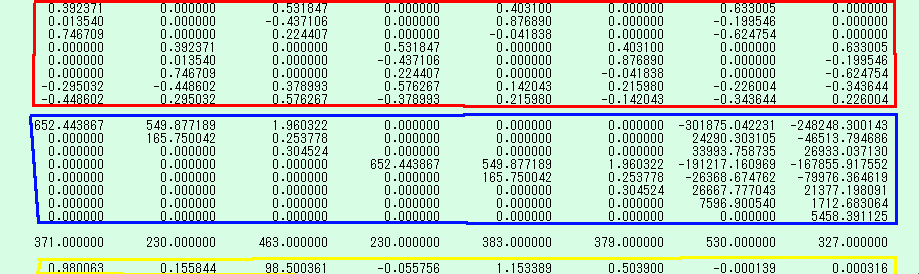
\includegraphics[scale=.5]{./img/fig2.png}

\section{[3.2] c言語での実装}

まず,QR分解するMatrixQRDecompColMajor関数と
交代代入をするMatricSimeqLr関数は以下のように実装した.

\begin{lstlisting}
void MatrixQRDecompColMajor(Matrix* mtR, Matrix* mt) {
    // Gram-Schmidt orthonormalization (R and Q)
    double t, * aT[] = { Row(mt,0), Row(mt,1), Row(mt,2), Row(mt,3), Row(mt,4), Row(mt,5), Row(mt,6), Row(mt,7) };
    int W = mt->W;
    MatrixClear(mtR);

    int i, j;
    for (i = 0; i < 8; i++) {
        for (j = 0; j < i; j++) {
            Elem(mtR, j, i) = t = VP(aT[j], aT[i], W);
            VSA(aT[i], aT[j], -t, W);
        }
        Elem(mtR, i, i) = t = sqrt(VP(aT[i], aT[i], W));
        VSS(aT[i], 1 / t, W);
    }

}

void MatrixSimeqLr(Matrix* mtB, Matrix* mtR) {
    // B = B L^{-1}
    double* B = Row(mtB, 0);
    double tmp;
    int i, j;
    for (i = 7; i >= 0; i--) {
        tmp = B[i];
        for (j = i+1; j <= 7; j++) {
            tmp -= B[j] * Elem(mtR, i, j);
        }
        B[i] = tmp / Elem(mtR, i, i);
    }
}
\end{lstlisting}

どちらも行列の大きさが変わったとき,for文の繰り返しの回数を変えることで対応可能にした.

\section{[3.3]}

次に,前回作成した投資投影画像を重ね合わせるプログラムで今回作成した射影変換行列を算出する
処理を呼び出すことで一つのプログラムにまとめた.
また,特徴点座標を改め一つにまとめたプログラムで生成された画像を以下に示す.

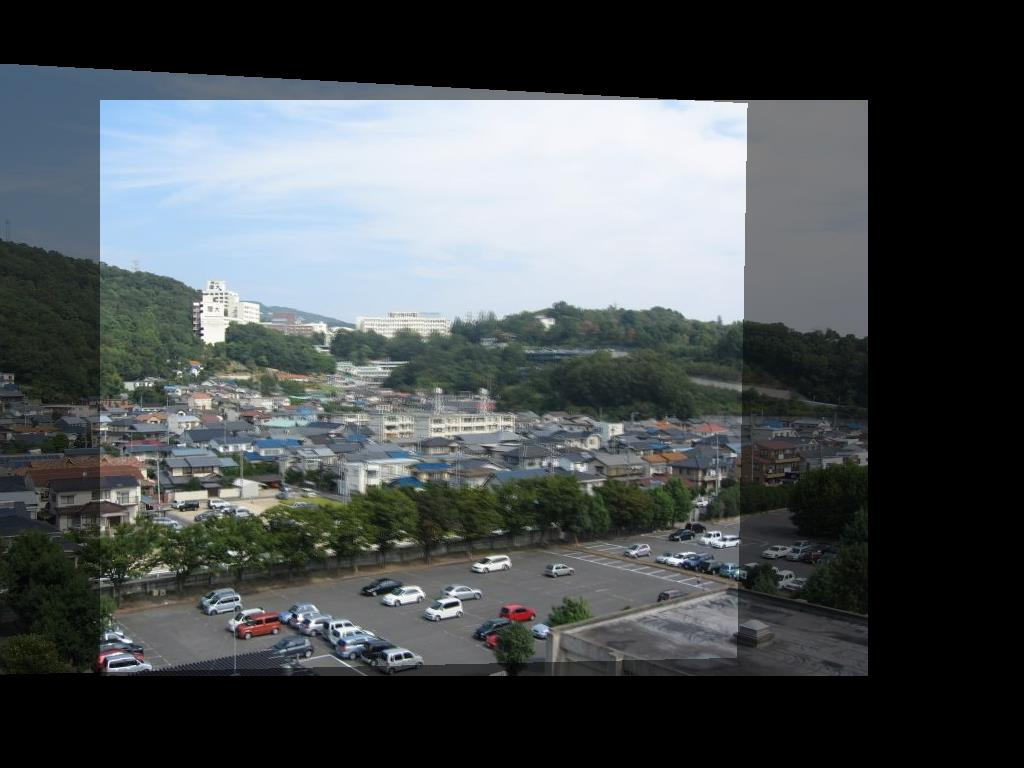
\includegraphics[scale=.4]{./img/out.jpg}

自分で撮影した画像を合成した結果を以下に示す.

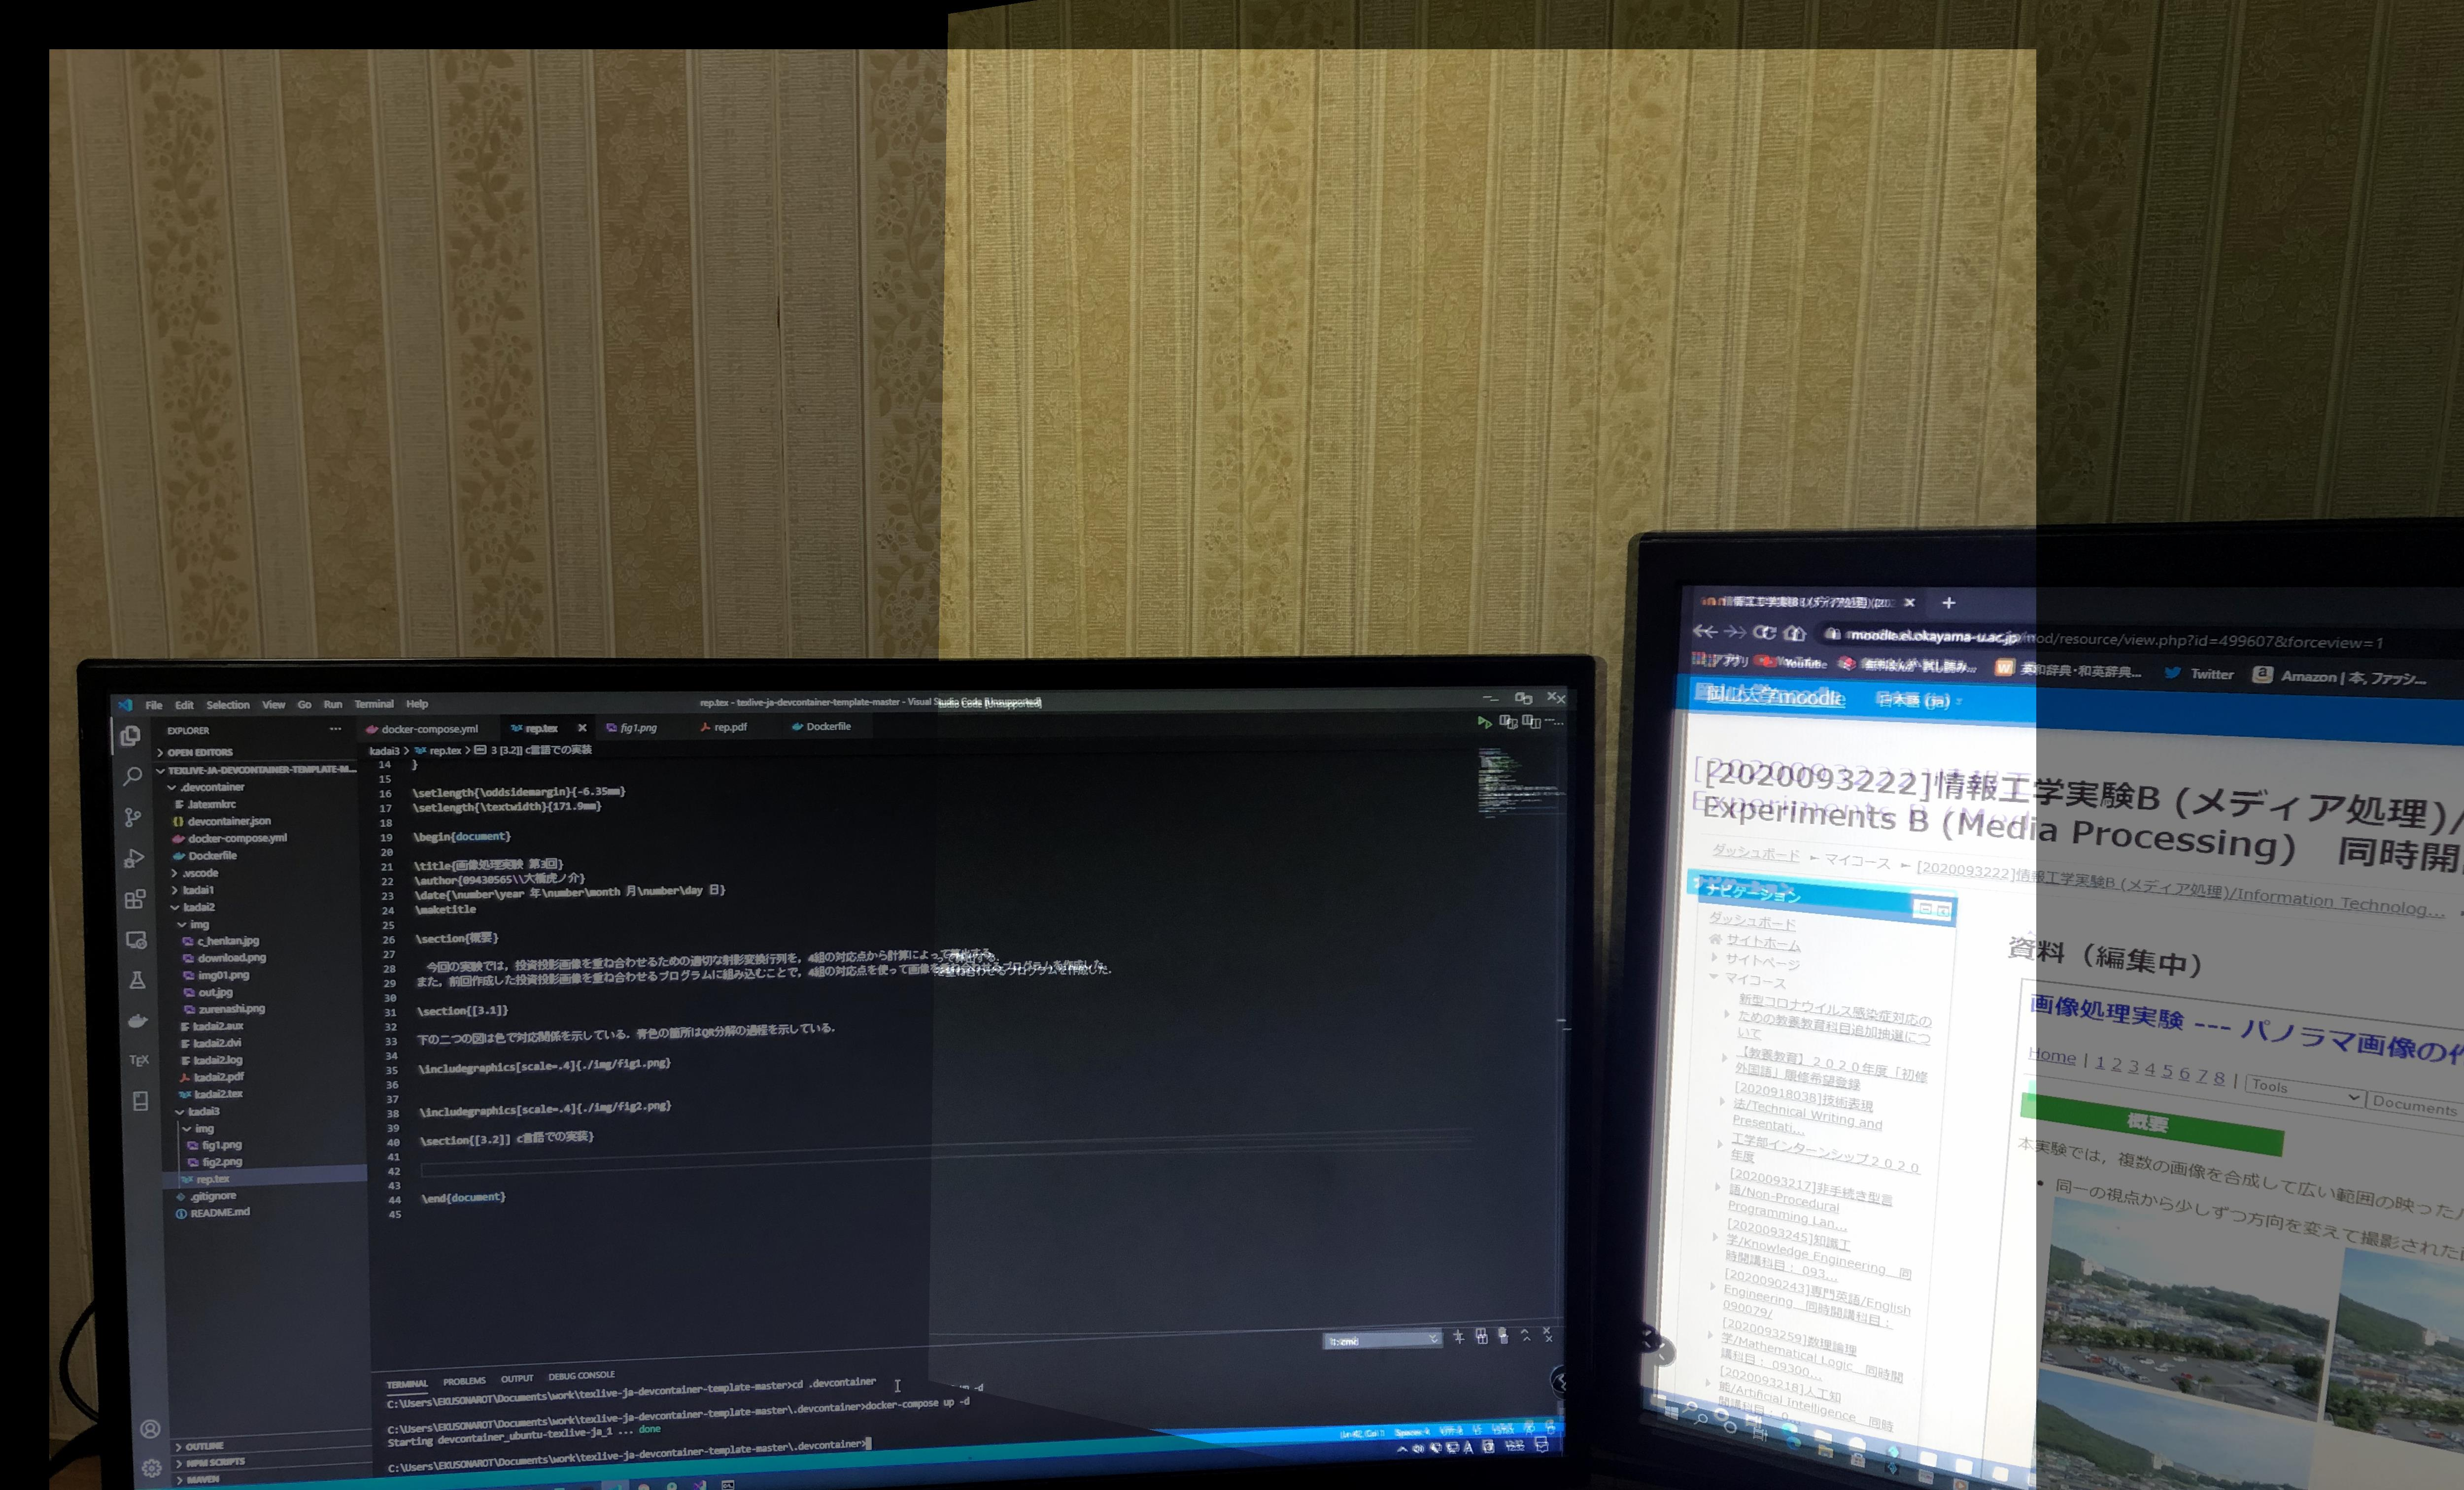
\includegraphics[scale=.1]{./img/tesktop.jpg}

\section{考察}

[3.3]で出力された画像は,第二回で出力されたものと比べて,うまく重なっている部分が
多いという印象を受ける.しかしこれはプログラムを変えたことや射影変換行列を計算で
求めるプログラムは関係なく,対応する特徴点が正確だったからである.

自分で撮影した画像を合成した画像は,少しずれているように感じる.
特徴点は離れた場所をとるほど,正確に合成できるが,この2枚の画像は共有部分が
狭かったので,離れた特徴点を選ぶことができなかった.
パノラマ撮影をする場合は,共通部分が多くなるようにたくさんの画像を使う方が
よいだろう.

\end{document}
